\documentclass[a4paper,12pt]{report}

\usepackage{cmap}
\usepackage[T2A]{fontenc}
\usepackage[utf8]{inputenc}
\usepackage[english,russian]{babel}
\usepackage{listings}
\usepackage{amsmath}
\usepackage{float}
\usepackage{csquotes}

\usepackage{xcolor}
\usepackage{hyperref}

\usepackage{graphicx}

\definecolor{dkgreen}{rgb}{0,0.6,0}
\definecolor{gray}{rgb}{0.5,0.5,0.5}
\definecolor{mauve}{rgb}{0.58,0,0.82}

\lstset{
    language=Python,            
    basicstyle=\small\sffamily, 
    numbers=left,           
    numberstyle=\tiny,       
    stepnumber=1,                  
    numbersep=5pt,               
    aboveskip=3mm,
    belowskip=3mm,
    showstringspaces=false,
    columns=flexible,
    captionpos=b, 
    basicstyle={\small\ttfamily},
    numbers=left,
    numberstyle=\tiny\color{gray},
    keywordstyle=\color{blue},
    commentstyle=\color{mauve},
    stringstyle=\color{dkgreen},
    breaklines=true,
    breakatwhitespace=true,
    tabsize=3
}

\title{Лабораторная работа №1\\Звуки и сигналы}
\author{Смирнов Никита}
\date{\today}

\begin{document}

\maketitle
\tableofcontents
\listoffigures
\lstlistoflistings

\maketitle

\chapter{Упражнение 1.1}

В данном упражнении нам нужно открыть \texttt{chap01.ipynb}, прочитать пояснения и  запустить примеры. Поэтому я просто изучил все примеры с комментариями. 

\chapter{Упражнение 1.2}
\section{Скачивание звука и работа с ним}

С предложенного нам сайта скачан звук проезжающей машины. Ссылка на соответствующий звук:

\href{https://freesound.org/people/gmetaxas/sounds/347662/}{https://freesound.org/people/gmetaxas/sounds/347662/}.

Далее звук был загружен, прослушан, и получена его визуализация.

\begin{lstlisting}[caption=Загрузка и прослушивание звука]
wave = thinkdsp.read_wave('347662__gmetaxas__motor-sound-road-no-effect.wav')
wave.normalize()
wave.make_audio()
\end{lstlisting}

\begin{lstlisting}[caption=Визуализация звука]
wave.plot()
\end{lstlisting}

\begin{figure}[H]
        \centering
        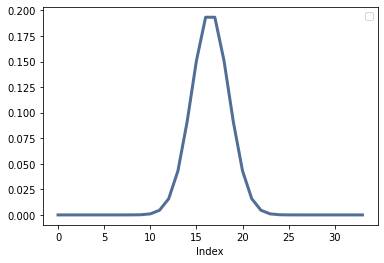
\includegraphics[width=0.75\textwidth]{1.png}
        \caption{Исходный звук}
        \label{fig: fig2_1}
\end{figure}
    
Берем полусекундный сегмент.

\begin{lstlisting}[caption=Изменение и прослушивание звука]
segment = wave.segment(start=1, duration=2)
segment.make_audio()
\end{lstlisting}

\begin{lstlisting}[caption=Визуализация укороченного звука]
segment.plot()
\end{lstlisting}

\begin{figure}[H]
        \centering
        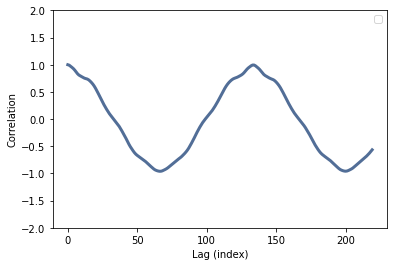
\includegraphics[width=0.75\textwidth]{2.png}
        \caption{Исходный звук}
        \label{fig: fig2_2}
\end{figure}

\section{Спектр звука}

Теперь рассмотрим спектр нашего полусекундного сегмента звука.

\begin{lstlisting}[caption=Спектр сегмента звука]
spectrum = segment.make_spectrum()
spectrum.plot(high=5000)
\end{lstlisting}

\begin{figure}[H]
        \centering
        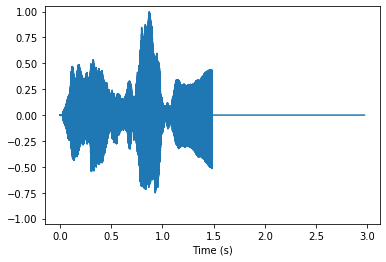
\includegraphics[width=0.75\textwidth]{3.png}
        \caption{Спектр сегмента звука}
        \label{fig:fig2_3}
\end{figure}

Увеличим маштаб.

\begin{lstlisting}[caption=Основные и доминирующие частоты]
spectrum = segment.make_spectrum()
spectrum.plot(high=1000)
\end{lstlisting}

\begin{figure}[H]
        \centering
        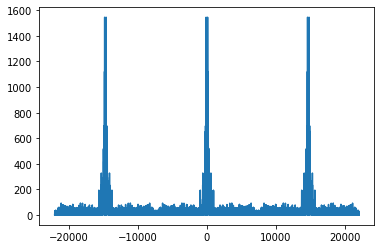
\includegraphics[width=0.75\textwidth]{4.png}
        \caption{Увеличиный маштиаб}
        \label{fig:fig2_4}
\end{figure}

\section{Фильтрация звука}

Применим фильтр нижних частот.

\begin{lstlisting}[caption=Фильтрация и воспроизведение звука]
spectrum.low_pass(400)
spectrum.make_wave().make_audio()
\end{lstlisting}

\begin{lstlisting}[caption=Визуализация фильтрации]
spectrum.make_wave().plot()
\end{lstlisting}

\begin{figure}[H]
        \centering
        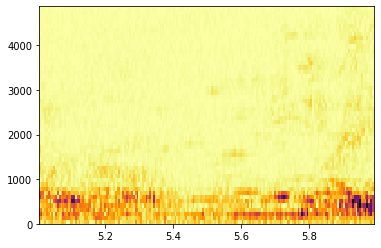
\includegraphics[width=0.75\textwidth]{5.png}
        \caption{Спектр сегмента звука}
        \label{fig:fig2_5}
\end{figure}

Видно, что график изменился, а звук стал, как из туннеля.

\chapter{Упражнение 1.3}
\section{Создание сложного сигнала}

Нужно создать сложный сигнал из объектов \texttt{SinSignal} и \texttt{CosSignal}.

\begin{lstlisting}[caption=Создание сложного сигнала из 4 элементов]
import thinkdsp

signal = (thinkdsp.SinSignal(freq=300, amp=0.1) + thinkdsp.SinSignal(freq=400, amp=1.5) +
thinkdsp.CosSignal(freq=300, amp=1.5) + thinkdsp.CosSignal(freq=100, amp=1.8))
signal.plot()
\end{lstlisting}

\begin{figure}[H]
        \centering
        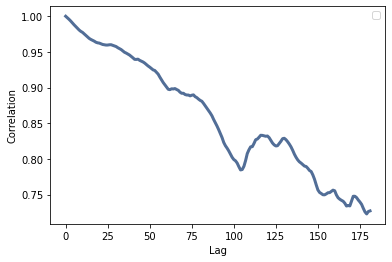
\includegraphics[width=0.75\textwidth]{6.png}
        \caption{Спектр сегмента звука}
        \label{fig:fig3_1}
\end{figure}

Теперь нужно получить звук.

\begin{lstlisting}[caption=Воспроизведение сложного сигнала]
wave = signal.make_wave(duration=2)
wave.apodize()
wave.make_audio()
\end{lstlisting}

Наж звук схож со звуком при звонке. Выведем спектр полученного звука.

\begin{lstlisting}[caption=Визуализация сигнала]
spectrum = wave.make_spectrum()
spectrum.plot(high=1000)
\end{lstlisting}

\begin{figure}[H]
        \centering
        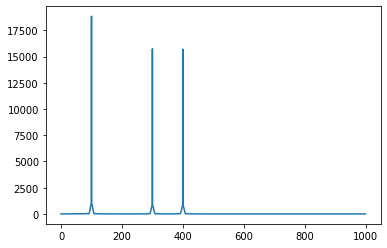
\includegraphics[width=0.75\textwidth]{7.png}
        \caption{Визуализация сегмента звука}
        \label{fig:fig3_2}
\end{figure}

\section{Добавление новой частоты}

Изменим наш сигнал.

\begin{lstlisting}[caption=Добавление новой частоты и воспроизведение]
signal += thinkdsp.SinSignal(freq=1000)
signal.make_wave().make_audio()
\end{lstlisting}

Теперь слышно добавленную новую частоту, при чём более высокую, потому что \texttt{freq=1000}. Теперь звук более похож на набор цифр при звонке через стационарный телефон.

\chapter{Упражнение 1.4}

Подготовим звук.

\begin{lstlisting}[caption=Загрузка и прослушивание звука]
wave = thinkdsp.read_wave('sounds/414062__felix-blume__machine-gears.wav')
wave.normalize()
wave.make_audio()
\end{lstlisting}

Теперь сделаем функцию \texttt{stretch}.

\begin{lstlisting}[caption=Функция stretch]
def stretch(wave, factor):
    wave.ts *= factor
    wave.framerate /= factor
\end{lstlisting}

Попробуем прослушать полученный звук, введя 0.25.

\begin{lstlisting}[caption=Прослушивание ускоренного звука]
stretch(wave3, 0.25)
wave.make_audio()
\end{lstlisting}

По таймеру в колабе время сократилсь с 5 до 2 секунд.

\begin{lstlisting}[caption=Визуализация ускоренного звука]
wave.plot()
\end{lstlisting}

\begin{figure}[H]
        \centering
        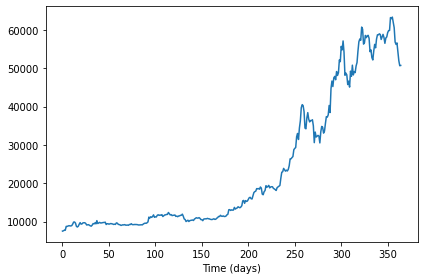
\includegraphics[width=0.75\textwidth]{8.png}
        \caption{Визуализация ускоренного звука}
        \label{fig:fig4_1}
\end{figure}

\chapter{Выводы}

Во время выполнения лабораторной работы получены навыки работаты со звуками, волнами и спектрами.

\end{document}
